%%% Here comes PPM's TeX template of 3/12/99. (templates/mathtplt.tex)%%%

\section{Determinant computation: Generic structure theorem method}  \label{ss:gdTL}
%{{{ gs thm approach

Our next method for computing the
Temperley--Lieb standard 
gram determinant
$\det(M_n(\lambda ))$
uses the generic structure theorem \cite[Th.1]{Martin91}. 
(Let us reiterate that there is no need, in representation theory, 
to compute any but the
elementary $\lambda=n-2$ case. We continue merely as an exercise in
service of later generalisations.)

The theorem gives a basis of the TL algebra for generic parameter
over a suitable field in the form of a complete
orthonormal set for the multimatrix structure.
In this case we can extract a basis for each cell module such %, of course, 
that, by orthonormality, the gram matrix is the unit matrix. 
Unlike the gram matrix over the defining `diagram' basis, this is of no
intrinsic use:  
manifestly since it contains no information; but implicitly
since we cannot specialise the 
parameter as we can if we work over the `integral' (polynomial) ring.
The trick is to keep track of the renormalisations of elements 
in passing from the integral basis, so that we can reconstruct
the determinant over the integral basis.  

The basis elements we need are defined as follows
(we extract directly from \cite[\S6.4]{Martin91}).

To start with, 
fix a standard/cell module $\Delta_n(\lambda)$ and consider the walk 
enumeration of the diagram basis. 
This consists of 
walks 
%$s=(s_1, s_2, ..., s_{n+1})$ 
$s=(s_0,s_1, s_2, ..., s_{n})$ 
of length $n$ on the positive part of the integral line
that start at 1 and end at $\lambda+1$.
The `lowest' walk can be depicted:
\[
e_m \; = \; 12121212123...m \; = \; 
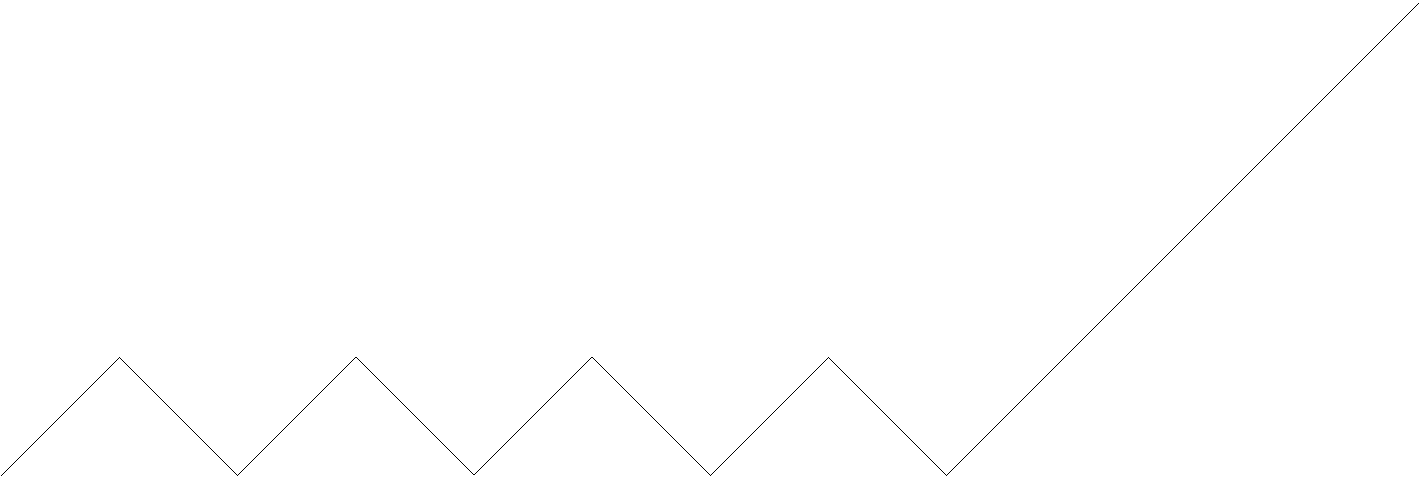
\includegraphics[width=4cm]{tex2/xfig-gramdetbyGST/d121212123456.pdf}
\]
where $m=\lambda+1$, for example. 
We will recall the correspondence between diagrams and walks shortly. 

Algebra basis elements correspond to pairs of these walks to the same endpoint, 
for all possible endpoints. 
Thus
with the endpoints running over the  $ \lambda \mapsto m=\lambda+1$ shifted possible 
cell module indices $\lambda$. Recall the $\lambda$s are  $n,n-2,...,0/1$, 
so we have  these shifted to $n+1,n-1,...,1$ or $...,2$. 

The map from pairs of walks to algebra elements can be given iteratively. 
Firstly the lowest walk (pair) for each $\lambda$ is mapped to 
an element by, for example with $m=\lambda+1$: 
\[
(e_m, e_m) = (121212123...m,121212123...m) = U_1 U_3 U_5 E_{m}^{(6)}
\]
(see \cite[\S6.4]{Martin91} for notation) (note normalisation as
idempotent needed). 
Then if $s_i =g-1$ is a minimum of
sequence $s$, and $s^i$ denotes $s$ with $s_i$ replaced by $g+1$:
\[
(s^i,t) = \; \sqrt{k_g k_{g+1}} \left( 1-\frac{U_i}{k_g} \right) (s,t)
\]
where $k_g = \frac{[g-1]}{[g]}$. 
And similarly on the right. 

The generic structure theorem \cite[\S6.4]{Martin91} ensures that these elements are an orthonormal basis of the TL algebra. 

The integral/diagram basis can be considered to start with 
$(e_m,e_m)$ (up to quotients and id normalisation - again see \cite{Martin91}). 
The next diagram basis element, corresponding to the walk 
$123212123...m$, is
$U_2 (e_m,e_m)$; 
and more generally $(s^i,t)_{diagram} = U_i (s,t)_{diagram}$. 
Thus we see that the new orthonormal basis element $(s^i,t)$ in this
case is got by adding a scalar multiple of the previous  %first 
(irrelevant for the determinant);
and rescaling   $U_i (s,t)$  %the second 
by 
\[
- \sqrt{\frac{[h-1]}{[h+1]}} \frac{[h]}{[h-1]}  \; =  \; - \sqrt{\frac{[h]^2}{[h+1][h-1]}}
\]
($h=g$).
This applies both to the bra and the ket, and both rescale the determinant. 
For a general walk there is a factor like this for each diamond added
to get to it from the $121212123...m$ walk.
Thus altogether we have the following. 

\begin{lem}
Schematically, 
\[
\det(M_n(\lambda)) = \prod_s \prod_d {\frac{[h]^2}{[h+1][h-1]}}
\]
where the products are over the set of walks and the diamonds in each
walk. 
\qed
\end{lem}

Example: The factors for each diamond are (in abridged notation):
\[
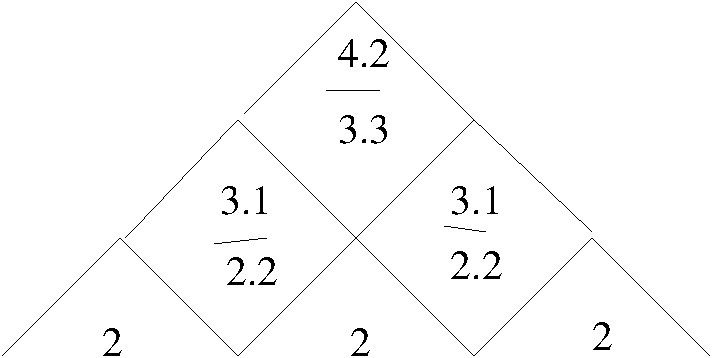
\includegraphics[width=4.47cm]{tex2/xfig-gramdetbyGST/d60b-eps-converted-to.pdf}
\]
Thus in particular
\[
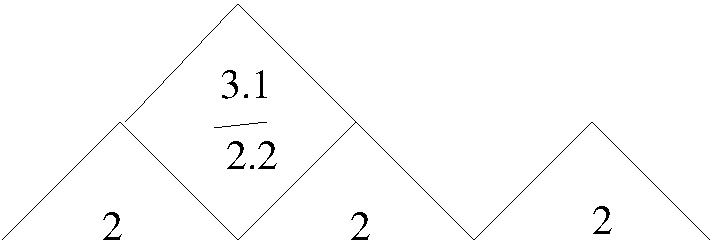
\includegraphics[width=4.47cm]{tex2/xfig-gramdetbyGST/d60b1232121-eps-converted-to.pdf}
\]
gives a factor $\frac{[3][2]}{1}$. Altogether we have
\[
\det( M_6(\lambda=0 )) = \frac{[2]^3}{1}
    \frac{[3][2]}{1} \frac{[3][2]}{1} \frac{[3]^2}{[2]^{}} \frac{[4]}{1} 
 = [2]^4 [3]^4 [4]
 = \delta^5 (\delta^2 -1)^4 (\delta^2 -2)
\]

Example II:
\[
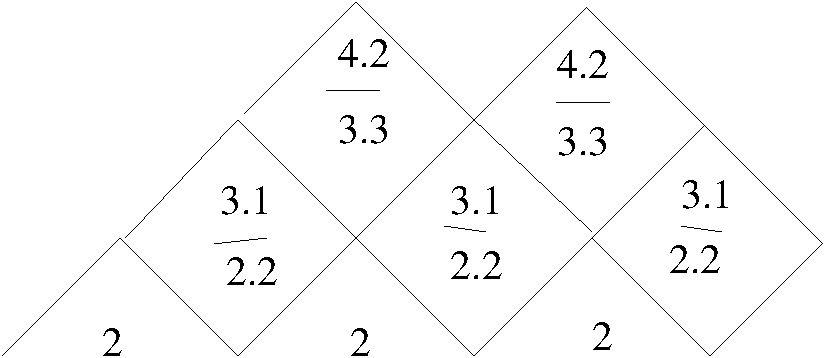
\includegraphics[width=5.37cm]{tex2/xfig-gramdetbyGST/d71x1-eps-converted-to.pdf}
\]
gives a factor $\frac{[4]^2 }{[2][3]}$. Altogether this det comes out as
\[
\det( M_7(\lambda=1 )) = \frac{[2]^{3\times 14}}{1}
    \left( \frac{[3]   }{[2]^2} \right)^{9+10+9} 
    \left( \frac{[4][2]}{[3]^2} \right)^{4+4}
    \left( \frac{[5][3]}{[4]^{2}} \right)^{1} 
 = [2]^{-6} [3]^{13} [4]^6 [5]
% = \delta^5 (\delta^2 -1)^4 (\delta^2 -2)
\]

Observe that the determinants can be computed recursively.
The walks that pass through $(\lambda-1,n-1)$ do not pick up another diamond in the final step, so contribute a factor $ det(M_{n-1}(\lambda-1)) $;
and those that pass $(\lambda+1,n-1)$ all pick up the same string of diamonds,
compared to their contribution to $ det(M_{n-1}(\lambda+1)) $. 
For example:
\[ { } \hspace{-.32in} 
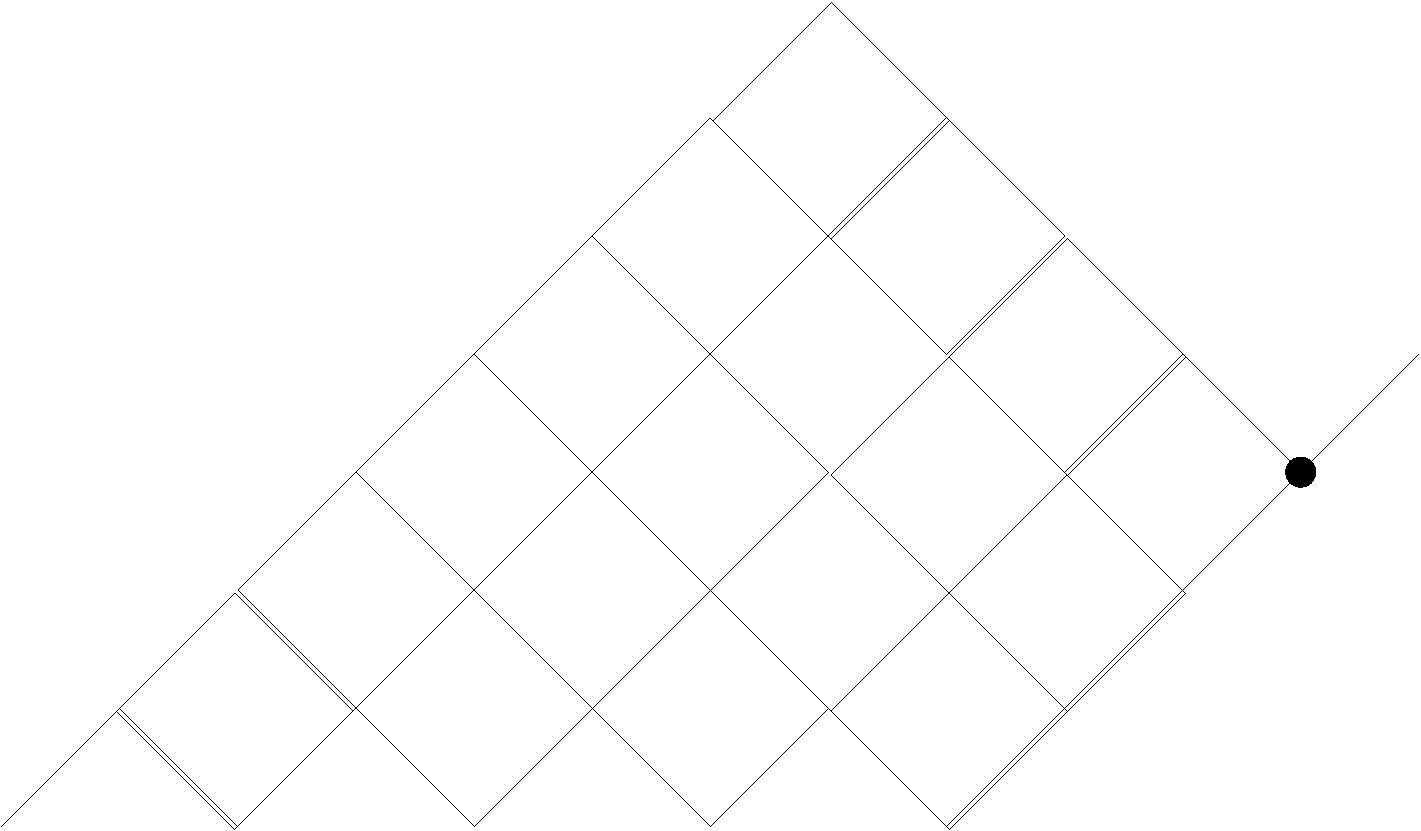
\includegraphics[width=5.4cm]{tex2/xfig-gramdetbyGST/d121212123456x2.pdf}
\qquad
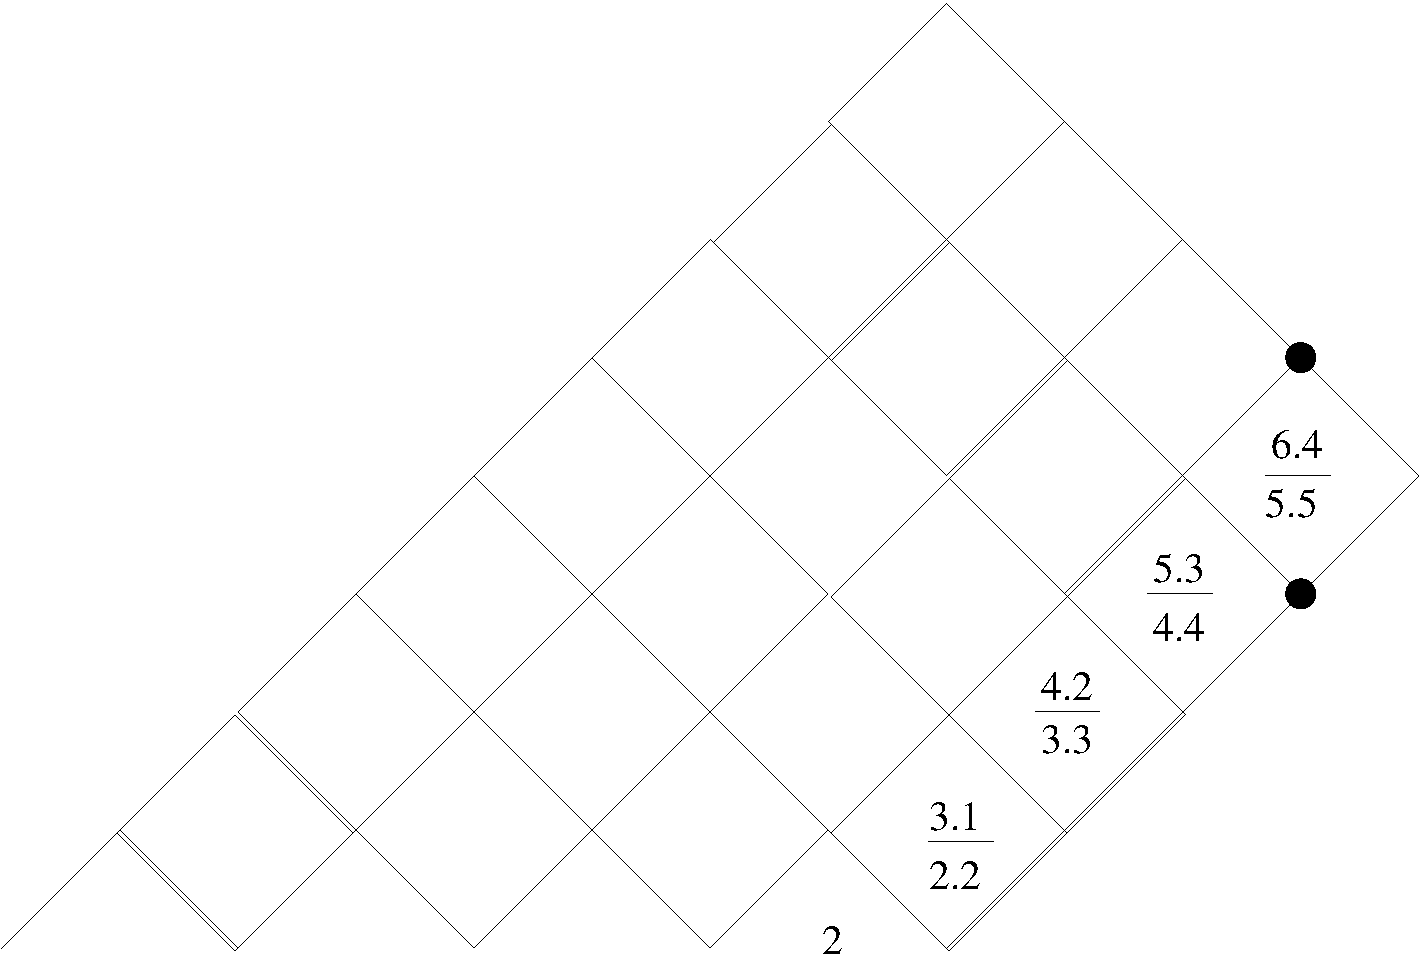
\includegraphics[width=5.4cm]{tex2/xfig-gramdetbyGST/d121212123456x.pdf}
\qquad
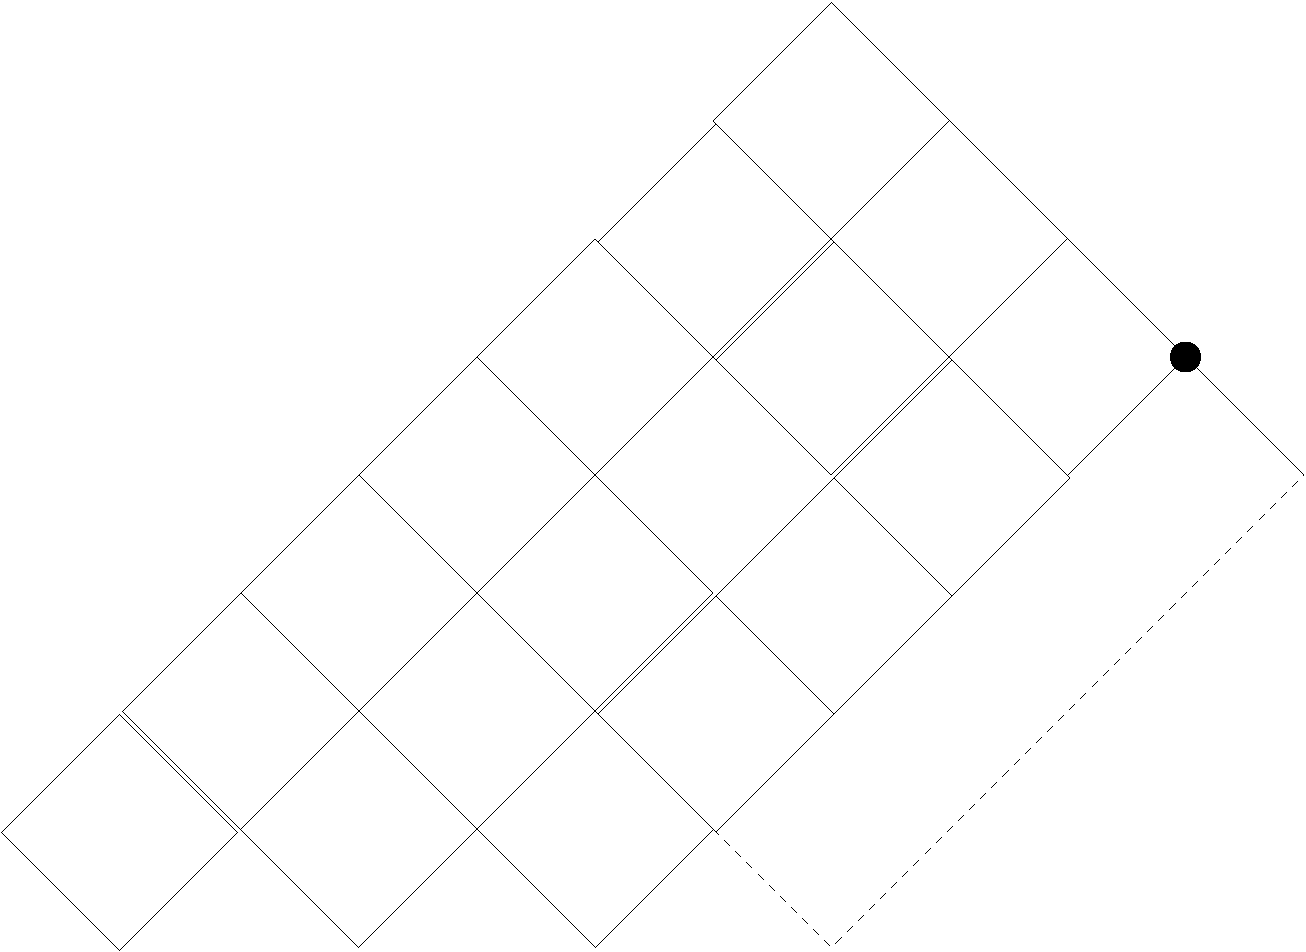
\includegraphics[width=5.04cm]{tex2/xfig-gramdetbyGST/d121212123456x3.pdf}
\]
We have
\beq \label{eq:det-recurs}
det(M_n(\lambda)) \;\; = \;\;\;\;
   det(M_{n-1}(\lambda-1)) \;\; . \;\;\;
    F_n(\lambda+1)^{dim(M_{n-1}(\lambda+1))} . det(M_{n-1}(\lambda+1))
\eq 
where the diamond-string factor is given by 
$$
F_n(\lambda) \;=\; [2] \frac{[3].1}{[2].[2]} \frac{[4].[2]}{[3].[3]} \frac{[5].[3]}{[4].[4]}
                     ... \frac{[\lambda+1].[\lambda-1]}{[\lambda].[\lambda]}
             \;\; = \; \frac{[\lambda+1]}{[\lambda]}
$$
% (using  the figure notation in the middle)
             - note that it does not actually depend on $n$.


Example:
\[
det(M_5(1)) \; =\;\; det(M_4(0))\;.F_5(2)^{dim(M_4(2))}.\; det(M_4(2))
            \; = \; [2]^2 [3] . \left( \frac{[3]}{[2]}\right)^{3} . [4]
            = \; \frac{[4][3]^4}{[2]}
\]

%}}}
%{{{ fig:bratelli5r2newX

%%  the following fig is created in xfig and exported to latex.
%%  (it looks like the Export option is the bare Latex one, not latex+eepic)
%%  to see the whole fig run   latex blobnotes3  (not pdflatex ...);
%%  then (on machine without dvipdf) dvipdfmx blobnotes3.
%%  need the macros too:
\def\qqt(#1,#2,#3){$q^{#1}[2]^{#2}[3]^{#3}$}
\def\qqf(#1,#2,#3,#4){$q^{#1}[2]^{#2}[3]^{#3}[4]^{#4}$}
\def\qqv(#1,#2,#3,#4,#5){$q^{#1}[2]^{#2}[3]^{#3}[4]^{#4}[5]^{#5}$}

\ignore{{ 
\begin{figure}
\input \xfigdd/bratelli5r2new2.latex
\caption{Specht Gram determinant data on Young graph
  (unfinished - reproduced from paper).
  NB this fig may work in dvi (latex ... compile)
  and not perfectly in pdf (pdflatex ...);
  but can run dvipdf or dvipdfmx on the dvi for a pdf file.
  %\label{fig:GY}
\label{fig:bratelli5r2new}}
\end{figure}
%
%\input xfig/bratelli5r2new.eepic  %% this seems to work even worse with pdflatex
}}

\ignore{\begin{figure} \vspace{-1cm} 
  %% the following invokes \includegraphics{....pdf};
  %% latexthrows a pdf bounding box issue, but you can keep going, or pdflatex:
%  \input xfig-bratelli5/bratelli5r2newa.pdf_t
  \input \xfigdd/bratelli5r2newa.pdf_t
  \caption{Specht Gram determinant data on Young graph
    (unfinished - reproduced from paper; some later $q^i$ factors omitted,
    but $q$ is a unit here so these are not relevant;
    the hook lengths shown are also not particularly relevant here).
    \label{fig:stray1}}
\end{figure}}

%% can't handle the colors etc:
%\input xfig-bratelli5/bratelli5r2new3.latex
%
%\input xfig-bratelli5/bratelli5r2new3.eepic

\ignore{\begin{figure} \vspace{-1cm} 
  %% the following invokes \includegraphics{....pdf};
  %% throws a pdf bounding box issue, but you can keep going:
%  \input xfig-bratelli5/bratelli5r2new3.pdf_t
  \input \xfigdd/bratelli5r2new3.pdf_t
  \caption{Coloured streaks indicate fibres projected to single point
    in TL global limit. \label{fig:streaky1}}
\end{figure}}

%% can't handle the in-fig latex:
%\includegraphics{xfig-bratelli5/bratelli5r2new3.eps}

%% can't handle the lack of pdf bounding box:
%\clearpage  \newpage { } \vspace{2in}
%
%\includegraphics{xfig-bratelli5/bratelli5r2new3.pdf}

%}}}
%{{{ fig:gramdetsXX

Now let us arrange the TL part of the result so that
the fibres are in vertical array under their $sl_2$ label
(and hence under the appropriate label in the projected Bratelli diagram): 
\[
\begin{array}{ccccccccccc}
  \lambda=0         &  1             &  2      &  3  &  4  &  5   %\hline
  \\ \hline
  1 \\ 
                   & 1  \\ 
   {[2]}           &                    & 1 \\ 
                  & [3]                &     & 1   \\ 
  {[ 2]}^2 [3]    &                     & [4] &      &  1  \\
                  & {[2]}^{-1} [3]^4 [4] &     & [5]   &    & 1 \\ 
{[2]}^4 [3]^4 [4]  &                    & {[2]}^{-1}[4]^5[5] &    & [6] & & 1 
\end{array}
\]
It is convenient to augment to also show the module dimensions (in red):
Fig.\ref{fig:gramdets01}.
And in Fig.\ref{fig:gramdets031} we include a schematic indication of the
recursive calculations from (\ref{eq:det-recurs}). 

\newcommand{\du}[2]{\begin{array}{c} \textcolor{red}{{#1}} \\ \hspace{-.321in}{#2}\hspace{-.321in} \end{array}}

\begin{figure}
  %
%\newcommand{\du}[2]{\begin{array}{c} \textcolor{red}{{#1}} \\ \hspace{-.321in}{#2}\hspace{-.321in} \end{array}}
%
%
%
\[ { } \hspace{-.53in} 
\begin{array}{ccccccccccccccccc}
%  \emptyset  & $\qed$ &  $\qed$ &  $\qed$ &  $\qed$ &  $\qed$ &  $\qed$ &  $\qed$ &   $\qed$ &   \\
  \lambda=0         &  1             &  2      &  3  &  4  &  5   & 6 & 7 & 8 
  \\ \hline
 \du{1}{1} \\ 
                  & \du{1}{1}  \\ 
 \du{1}{{[2]}}     &                  & \du{1}{1} \\ 
                  & \du{2}{[3]}                &     & \du{1}{1}   \\ 
 \du{2}{{[ 2]}^2 [3]}  &                     & \du{3}{[4]} &    & \du{1}{1}  \\
               & \du{5}{{\frac{ [3]^4 [4]}{[2]}^{}}} &  & \du{4}{[5]} &  & \du{1}{1} \\ 
 \du{5}{{[2]}^4 [3]^4 [4]} &              & \du{9}{{\frac{[4]^5[5]}{[2]}^{}}} &    & \du{5}{[6]} & & \du{1}{1}  \\
              & \du{14}{\frac{[3]^{13}[4]^6[5]}{[2]^{6}}} &&\du{14}{\frac{[5]^6[6]}{[2]^{}}} && \du{6}{[7]} && \du{1}{1}
 \\
 \du{14}{[2]^8[3]^{13}[4]^6[5]}  &&      \du{28}{\frac{[4]^{20}[5]^7[6]}{[2]^{7}[3]^{}}} && \du{20}{\frac{[6]^7[7]}{[2]^{}}} && \du{7}{[8]}  &&  \du{1}{1} \\
              & \du{42}{\frac{[3]^{40}[4]^{26}[5]^8[6]}{[2]^{27}}} && \du{48}{\frac{[5]^{27}[6]^8[7]}{[2]^{8}[3]^{}}} && \du{27}{\frac{[7]^8[8]}{[2]^{}}} && \du{8}{[9]} && \du{1}{1}
 \\
 \du{42}{[2]^{15}[3]^{40}[4]^{26}[5]^{8}[6]} && \du{90}{\frac{[4]^{74}[5]^{35}[6]^{9}[7]}{[2]^{35}[3]^{9}}} && \du{75}{
   %[4]^{0}[5]^{0}
 \frac{  [6]^{35}[7]^{9}[8]}{[2]^{9}[3]^{}}} && \du{35}{\frac{[8]^9[9]}{[2]^{}}} && \du{9}{[10]} && \du{1}{1}
\end{array}
\]


  \caption{Standard Gram determinants restricting to the TL weights and then organising by $sl_2$ labels.
%    \qquad 
%(The very top row of labels are for connecting to Brauer algebra rep theory and can be ignored here.)
    \label{fig:gramdets01}}
\end{figure}


\begin{figure}
  %
%\newcommand{\du}[2]{\begin{array}{c} \textcolor{red}{{#1}} \\ \hspace{-.321in}{#2}\hspace{-.321in} \end{array}}
\newcommand{\sqrr}{\square\ar[r]}
%
%
\[ { } \hspace{-.253in}
%
\xymatrix @C=15pt @R=1pt {
%  {\emptyset}\ar[r] & \sqrr & \sqrr & \sqrr & \sqrr & \sqrr & \sqrr & \sqrr & \sqrr & { }
%  \\
  {\lambda=0  }       &  1             &  2      &  3  &  4  &  5   & 6 & 7 & 8 
  \\  %\hline
    {\du{1}{1} }\ar[dr]
    \\
& {\du{1}{1}}\ar[dr]\ar[dl]^{2/1}
\\ 
{\du{1}{{[2]}} }\ar[dr]    &                  &
{\du{1}{1}}\ar[dr]\ar[dl]^{3/2}
\\
&{\du{2}{[3]}} \ar[dr]\ar[dl]^{2/1}               &     &
{\du{1}{1}}\ar[dr]\ar[dl]^{4/3}
\\ 
{ \du{2}{{[ 2]}^2 [3]}}  \ar[dr]  &                     &
{\du{3}{[4]} }  \ar[dr]\ar[dl]^{3/2}  &    &
{\du{1}{1} } \ar[dr]\ar[dl]^{5/4}
\\
    & {\du{5}{{\frac{ [3]^4 [4]}{[2]}^{}}}}  \ar[dr]\ar[dl]^{2/1}   &  &
    {\du{4}{[5]}} \ar[dr]\ar[dl]^{4/3} &  &
    {\du{1}{1}} \ar[dr]\ar[dl]^{6/5}
    \\ 
    {\du{5}{{[2]}^4 [3]^4 [4]}} &              &
    {\du{9}{{\frac{[4]^5[5]}{[2]}^{}}}} &    &
    {\du{5}{[6]}} & &{ \du{1}{1} }
    \\ 
    &{\du{14}{\frac{[3]^{13}[4]^6[5]}{[2]^{6}}}} &&
    {\du{14}{\frac{[5]^6[6]}{[2]^{}}}} &&
    {\du{6}{[7]}} &&
    {\du{1}{1}}
 \\
   {\du{14}{[2]^8[3]^{13}[4]^6[5]}}  &&
   {\du{28}{\frac{[4]^{20}[5]^7[6]}{[2]^{7}[3]^{}}}} &&
   {\du{20}{\frac{[6]^7[7]}{[2]^{}}}} &&
   {\du{7}{[8]}}  &&
   {\du{1}{1}} \\
   & {\du{42}{\frac{[3]^{40}[4]^{26}[5]^8[6]}{[2]^{27}}}} &&
   {\du{48}{\frac{[5]^{27}[6]^8[7]}{[2]^{8}[3]^{}}}} &&
   {\du{27}{\frac{[7]^8[8]}{[2]^{}}}} &&
   {\du{8}{[9]}} &&
   {\du{1}{1}}
 \\
   {\du{42}{[2]^{15}[3]^{40}[4]^{26}[5]^{8}[6]}}\ar[dr] &&
   {\du{90}{\frac{[4]^{74}[5]^{35}[6]^{9}[7]}{[2]^{35}[3]^{9}}}}\ar[dl]^{3/2} &&
   {\du{75}{
   %[4]^{0}[5]^{0}
       \frac{  [6]^{35}[7]^{9}[8]}{[2]^{9}[3]^{}}}} &&
   {\du{35}{\frac{[8]^9[9]}{[2]^{}}}} &&
   {\du{9}{[10]}} &&
   {\du{1}{1}}
   \\
   & { \begin{array}{c} { } \\ \textcolor{red}{132} \\ 
        {[2]^{15-90-35}} \\ {[3]^{40+90-9}} \\
        {[4]^{26+74}} \\ {[5]^{8+35}} \\ {[6]^{1+9}[7]}
        \end{array} }
}
\]


  \caption{The recursive construction for gram determinants, as in (\ref{eq:det-recurs}).
    The weightings
    $ ( [\lambda\!+\!1]/[\lambda] )^{dim(M_{n-1}(\lambda+1))} $
    are drawn simply as
    $\lambda\!+\!1/\lambda$. 
    We omit drawing edges after the various patterns are established,
    apart from the explicit calculation shown at the bottom. 
    \label{fig:gramdets031}}
\end{figure}

\ignore{\begin{figure}
  %
%\newcommand{\du}[2]{\begin{array}{c} \textcolor{red}{{#1}} \\ \hspace{-.321in}{#2}\hspace{-.321in} \end{array}}
\newcommand{\sqrr}{\square\ar[r]}
\newcommand{\goll}{\ar@/_1.3pc/[ll]} 
\newcommand{\gollll}{\ar@/_1.4pc/[llll]} 
\newcommand{\gollllll}{\ar@/_1.5pc/[llllll]} 
\newcommand{\gollllllll}{\ar@/_1.7pc/[llllllll]} 
%
%
\[ { } \hspace{-.253in}
%
\xymatrix @C=15pt @R=1pt {
%  {\emptyset}\ar[r] & \sqrr & \sqrr & \sqrr & \sqrr & \sqrr & \sqrr & \sqrr & \sqrr & { }
%  \\
  {\lambda=0  }       &  1             &  2      &  3  &  4  &  5   & 6 & 7 & 8 
  \\  %\hline
    {\du{1}{1} }\ar[dr]
    \\
& {\du{1}{1}}\ar[dr]\ar[dl]^{2/1}
\\ 
{\du{1}{{[2]}} }\ar[dr]    &                  &
{\du{1}{1}}\ar[dr]\ar[dl]^{3/2}
\\
&{\du{2}{[3]}} \ar[dr]\ar[dl]^{2/1}               &     &
{\du{1}{1}}\ar[dr]\ar[dl]^{4/3}
\\ 
{ \du{2}{{[ 2]}^2 [3]}}  &                     &
{\du{3}{[4]} }&    &
{\du{1}{1} }
\\
    & {\du{5}{{\frac{ [3]^4 [4]}{[2]}^{}}}} &  &
    {\du{4}{[5]}} &  &
    {\du{1}{1}}\ar@/_1.3pc/[ll]
    \\ 
    {\du{5}{{[2]}^4 [3]^4 [4]}} &              &
    {\du{9}{{\frac{[4]^5[5]}{[2]}^{}}}} &    &
    {\du{5}{[6]}} & &{ \du{1}{1}}\ar@/_1.4pc/[llll]
    \\ 
    &{\du{14}{\frac{[3]^{13}[4]^6[5]}{[2]^{6}}}} &&
    {\du{14}{\frac{[5]^6[6]}{[2]^{}}}} &&
    {\du{6}{[7]}}\ar@/_1.3pc/[ll] &&
    {\du{1}{1}}\gollllll
 \\
   {\du{14}{[2]^8[3]^{13}[4]^6[5]}}  &&
   {\du{28}{\frac{[4]^{20}[5]^7[6]}{[2]^{7}[3]^{}}}} &&
   {\du{20}{\frac{[6]^7[7]}{[2]^{}}}} &&
   {\du{7}{[8]}}\gollll  &&
   {\du{1}{1}}\gollllllll \\
   & {\du{42}{\frac{[3]^{40}[4]^{26}[5]^8[6]}{[2]^{27}}}} &&
   {\du{48}{\frac{[5]^{27}[6]^8[7]}{[2]^{8}[3]^{}}}} &&
   {\du{27}{\frac{[7]^8[8]}{[2]^{}}}}\goll &&
   {\du{8}{[9]}}\gollllll &&
   {\du{1}{1}}
 \\
   {\du{42}{[2]^{15}[3]^{40}[4]^{26}[5]^{8}[6]}} &&
   {\du{90}{\frac{[4]^{74}[5]^{35}[6]^{9}[7]}{[2]^{35}[3]^{9}}}} &&
   {\du{75}{
   %[4]^{0}[5]^{0}
       \frac{  [6]^{35}[7]^{9}[8]}{[2]^{9}[3]^{}}}} &&
   {\du{35}{\frac{[8]^9[9]}{[2]^{}}}}\gollll &&
   {\du{9}{[10]}}\gollllllll &&
   {\du{1}{1}}\goll
}
\]


  \caption{\ppm{[NB this is a duplicate since we already copied in this fig earlier as \ref{fig:gramdets03--}!]}
  Standard to standard module maps when $[5]=0$.
    This is perhaps best viewed alcove-geometrically - the ambient space is $\R$;
    the origin is at $\lambda=-1$ (it is `$\rho$-shifted');
    and the first affine wall at $\lambda=-1+5=4$.  \label{fig:gramdets03}}
\end{figure}}

At its most succinct this scheme can be reduced to:
\[
\xymatrix@C=45pt{
  %\lambda=
  0  \ar@<.31ex>[r]^1   &
  1 \ar@<.31ex>[r]^1 \ar@<.21ex>[l]^{{{ } \;\; [2]/1}}    &
  2 \ar@<.31ex>[r]^1 \ar@<.21ex>[l]^{[3]/[2]}   &
  3 \ar@<.31ex>[r]^1 \ar@<.21ex>[l]^{[4]/[3]}  &
  4  \ar@<.21ex>[l]^{[5]/[4]}  &
  \cdots
}
\]
meaning that $det(M_n(\lambda))$ is the product of the $det(M_{n-1}(\mu))$'s
corresponding to the incoming arrows
(the $\lambda,\;\mu$ labels are on the vertices);
together with the factors {\em on}
the incoming arrows raised to the power of $dim(M_{n-1}(\lambda+1))$. 


\medskip \vspace{.5in} 

%}}}
%{{{ JOB

\noindent 
%JOB: show
To see how these determinants check against representation theory,
consider for example Fig.\ref{fig:gramdets03}.
Here we focus on the parameter value such that $[5]=0$.
The first determinant that vanishes is then indicated in the figure.
This vanishing indicates that there is a non-isomorphism map from
the corresponding costandard module to the standard module;
and hence that the standard module has a socle.
In this case it is one-dimensional and it is straightforward to deduce that
this corresponds to a map in from the trivial module.
--- And this is what the curved arrow indicates.

In the next layer we see a similar vanishing; and deduce a similar map.

In the next layer we have another. But we also have a globalisation image of
the very first map - where the module mapping in is
the globalisation image of the trivial, and so 
not the trivial.
Note that this has a direct affect on the degree of vanishing of the determinant (recall we have connected this to the Smith form of the gram matrix). 

Hopefully the subsequent pattern will be clear.
Perhaps the next interesting observation is in the last rank shown.
Here we have a map from the trivial module (of course $[5]=0$ implies $[10]=0$);
and we already have an on-map, due to the globalisation property. 
By inspecting the degrees of vanishing of the various gram matrices we can
deduce that the composite map vanishes here.


%}}}
\vspace{.5cm}
\subsection{What about the Smith form?} 
%{{{ SNF
More than the determinant evaluated over the ground field of interest,
$K$ say,
one cares about the rank of the gram matrix
(evaluated over the ground field of interest).
This is because the rank
 determines the rank of the contravariant form, and hence
the dimension of the simple head of the cell module over $K$. 
Elementary row and column operations expressible as multiplication by 
invertible matrices do not change the rank. Thus, if we are working
over a PID (as we are in the indeterminate-$\delta$ calculations 
if the coefficient ring is a field)
we are interested in the Smith normal form (SNF).

Reduced to the ground field of interest the SNF will give the rank
directly.
(Even if the ground ring is not a PID there may be a form which
directly reveals the rank.)
(The SNF may reveal even more than the rank in general. 
The power of vanishing of
invariant factors vanishing   %%over the ground field
at the $\delta$-value 
of interest may reveal details of factor modules deeper in the
Jordan--Holder series of the cell module.) 

Example:
Consider the gram matrix
\[
\mat{cccc} \delta & 1 & 0 \\ 1 & \delta & 1 \\ 0 & 1 & \delta
\tam
\stackrel{R1:R1+R3}{\leadsto}
\mat{cccc} \delta & 2 & \delta \\ 1 & \delta & 1 \\ 0 & 1 & \delta
\tam
\stackrel{R1:R1-\delta R2}{\leadsto}
\mat{cccc} 0 & 2-\delta^2 & 0 \\ 1 & \delta & 1 \\ 0 & 1 & \delta
\tam
\stackrel{C2:C2-\delta C1;...}{\leadsto}
\]\[
\mat{cccc} 0 & 2-\delta^2 & 0 \\ 1 & 0 & 0 \\ 0 & 1 & \delta
\tam
\stackrel{R1:R1+(\delta^2 -2) R3}{\leadsto}
\mat{cccc} 0 & 0 & -\delta(2-\delta^2 )  \\ 1 & 0 & 0 \\ 0 & 1 & \delta
\tam
...
\]
We can compute the SNF in various ways. It is
\[
\mat{cccc} \delta (\delta^2 -2) && \\ &1& \\ &&1 \tam
\]
Method 1: elementary row and column operations.
\\
Method 2: compute minors and take the HCF of all minors at each rank. 
For example the HCF of $1\times 1$ minors in our example is clearly 1;
as is that of $2\times 2$ minors. The final invariant factor is then
forced. 




%}}}



%{{{ Local vars
% § Local Variables

% Local Variables:
% mode: LaTeX
% folded-file: t
% End:

% ¶
%}}}
